%auto-ignore
%      this ensures the arxiv doesn't try to start TeXing here.
%!TEX root = super_lattice_models_draft.tex
%      prev line helps TeXShop do the right thing

%%%%%%%%%%%%%%%%%%%%%%%%%%%%%%%%%%%%%%
\section{Fermion condensation in the Ising TQFT}  \label{C2_condense_sect}
%%%%%%%%%%%%%%%%%%%%%%%%%%%%%%%%%%%%%%

Before discussing super pivotal categories in the abstract and general techniques for constructing examples thereof,
we will give a detailed account of one of the simplest examples:
the $C_2$ super pivotal category.
This theory 
is obtained from the Ising TQFT by condensing the emergent fermion $\psi$, and provides a good demonstration of the 
qualitatively new features that occur as a result of fermion condensation. 
This section (and the next) is organized as follows: in \ref{Ising_review} we briefly review the aspects of the 
Ising TQFT we will need in later sections. 
In \ref{general_condensation} we comment on the general procedure of anyon condensation, and in \ref{condensing_psi} 
we show how to condense $\psi$ in the Ising theory, obtaining the $C_2$ super pivotal theory. 
\ref{C2_local_relns} details the diagrammatic properties of the $C_2$ theory, and in \ref{C2excitations} we compute 
the quasiparticle excitations of the theory. 
In \ref{C2_fusion_rules} we determine the fusion rules of these quasiparticles, and in \ref{C2_braiding} we compute 
their statistical and braiding data and analyze the modular $S$ and $T$ matrices in detail. 


%%%%%%%%%%%%%%%%%%%%%%%
\subsection{Ising TQFT}  \label{Ising_review}
%%%%%%%%%%%%%%%%%%%%%%%

Here we provide a brief review the the Ising TQFT (see e.g. \cite{Lins1994}). 
There are three particles in the theory, which we label as $\unit$ (the trivial particle), $\sigma$ 
(the non-abelian Ising anyon), and $\psi$ (the emergent fermion).
The nontrivial fusion rules of the theory are as follows:
\be 
	\sigma\tp\sigma\cong\unit\oplus\psi,\quad \sigma\tp\psi\cong\sigma,\quad\psi\tp\psi\cong\unit.
\ee

The quantum dimensions of the particles are 
\be
\label{QuantumDimensions}
d_\unit = 1 \quad d:=d_\sigma = -A^2 - A^{-2} \quad d_\psi =1,
\ee
where $A$ is a primitive 16th root of unity. Graphically, this means that
\begin{align}
\dpsi_\psi = \text{(vaccuum)} \qquad \qquad \dbeta_\beta = d \times \text{(vaccuum)}
\end{align}
where the blue (orange) circle denotes a circular $\psi$ ($\sigma$) worldline.
$\unit$ worldlines, being identified with the vaccuum, are not drawn in diagrams. 

Out of the eight possible choices for $A$, the four different choices $A = ie^{\pm i\pi/8}, -ie^{\pm i\pi/8}$ 
all give a positive quantum dimension for the $\sigma$ particle of $d = \sqrt{2}$.
The other four choices of $A$ give $d=-\sqrt{2}$, which can alternatively be defined
with $d=\sqrt{2}$ but with a negative Frobenius-Schur indicator of $\kappa_\sigma=-1$. 
In what follows, we will specify to $A = ie^{\pm i\pi/8}, -ie^{\pm i\pi/8}$ so that $d_\sigma = \sqrt{2},\kappa_\sigma=1$. 


We now turn our attention to the graphical calculus of the Ising TQFT. 
We pick a normalization more common in the physics literature,
bubbles in diagrams can be eliminated by using the rule
\be
\overset{\;c'}{\underset{c}{{\scriptstyle{a}}\Bubbleabc {\scriptstyle{b}}}} = \delta_{c c'} \sqrt{\frac{d_a d_b}{d_c}}\times \overset{c}{\underset{c}{\idblack}}\ee
In particular, we have 
\be
\overset{\sigma}{\underset{\sigma}{{\scriptstyle{\sigma}}\Bubblesps {\scriptstyle{\psi}}}} = \overset{\sigma}{\underset{\sigma}{\idorange}}\;, \quad \quad 
\overset{\sigma}{\underset{\sigma}{{\scriptstyle{\sigma}}\Bubblessp {\scriptstyle{\sigma}}}}
 = d \times \overset{\psi}{\underset{\psi}{\idblue}}\; ,
  \label{Ising_bubble_relns} 
\ee
where again, we are marking $\psi$ worldlines in dark blue and $\sigma$ worldlines in orange. 


The non-trivial $F$-moves in the theory are as follows:
\begin{align}	
& \IsingDat{\VssI}{\sigma}{\sigma}{\sigma}{\sigma}  =\frac{1}{d} \left(   \IsingDat{\HssI}{\sigma}{\sigma}{\sigma}{\sigma} + \IsingDat{\ScriptOverSymbol{\Hssp}{\substack{\; \\ \; \\ \psi }}}{\sigma}{\sigma}{\sigma}{\sigma} \right) \qquad \qquad
\IsingDat{\ScriptOverSymbol{\Vsps}{\;\; \;\; \sigma }}{\sigma}{\psi}{\sigma}{\psi} = 
 \IsingDat{\HspI}{\sigma}{\psi}{\sigma}{\psi}  \\[4ex]
& \IsingDat{\ScriptOverSymbol{\Vssp}{\;\; \;\; \psi }}{\sigma}{\sigma}{\sigma}{\sigma}  = \frac{1}{d} \left(   \IsingDat{\HssI}{\sigma}{\sigma}{\sigma}{\sigma} - \IsingDat{\ScriptOverSymbol{\Hssp}{\substack{\; \\ \; \\ \psi }}}{\sigma}{\sigma}{\sigma}{\sigma} \right) \qquad \qquad 
 \IsingDat{\VppI}{\psi}{\psi}{\psi}{\psi} =  \IsingDat{\HppI}{\psi}{\psi}{\psi}{\psi} 	
 \end{align} 
The twist and braiding of the $\sigma$ particle are given by 
\begin{align}
\underset{\;\;\; \; \;\;\;  \sigma }{\overset{\;\;\; \; \;\;\;  \sigma }{\Twists} } = -A^3\; \underset{\sigma}{\overset{\sigma}{\idsigmashort}}  \qquad \qquad 
\IsingDat{\Braidss}{\sigma}{\sigma}{\sigma}{\sigma} = A \: \IsingDat{\HssI}{\sigma}{\sigma}{\sigma}{\sigma} + A^{-1} \IsingDat{\VssI}{\sigma}{\sigma}{\sigma}{\sigma} 
\label{sigma_braiding}
\end{align}
The formula for the topological twist on the left follows from the relation given on the right.
Using that $\sigma \tp \sigma = \unit \oplus \psi$ and \eqref{sigma_braiding} 
we can derive the braiding data for the $\psi$ particle. 
Most importantly for us, the
$\psi$ particle is fermionic in both its topological twist 
and statistics, regardless of the choice of $A$:
\begin{align}
  \underset{\;\;\; \; \;\;\;  \psi }{\overset{\;\;\; \; \;\;\;  \psi }{\Twistp} }= -\;  \underset{\psi}{\overset{\psi}{\idpsishort}} \qquad \qquad \IsingDat{\Braidpp}{\psi}{\psi}{\psi}{\psi}  = (-1) \IsingDat{\HppI}{\psi}{\psi}{\psi}{\psi} 
\label{psi_a_fermion}
\end{align}
Additionally, $\psi$ is not transparent, as it braids nontrivially with $\sigma$:
\begin{align}
 \overset{\sigma \quad \; \; \; \; \psi }{\underset{\sigma}{\Rpss}}
 =A^4 \;  \overset{\sigma \quad \; \; \; \; \psi }{\underset{\sigma}{\Vsigmapsisigma}}, \qquad \qquad \IsingDat{\Braidsp}{\psi}{\sigma}{\sigma}{\psi}  = - \IsingDat{\Braidpsconj}{\psi}{\sigma}{\sigma}{\psi}. 
  \label{sig_psi_Rsymbol}
\end{align}

Our goal in what follows is to describe how to condense the $\psi$ particle in the Ising TQFT. 
To put this in context, we will first make a few remarks on the more familiar bosonic condensation. 






%%%%%%%%%%%%%%%%%%%
\subsection{Condensation of transparent bosons}\label{general_condensation}
%%%%%%%%%%%%%%%%%%%

We now briefly review how to perform condensation with transparent bosons (see e.g. \cite{eliens2014}).  
Let $\mcc$ be a ribbon category and let $\alpha$ be a particle (simple object) of $\mcc$ which we hope to condense.
In category theoretic terms, we want to add morphisms to $\mcc$ so that $\alpha$ becomes
isomorphic to the trivial particle $\unit$ (or, more generally, to a direct sum of several copies of $\unit$). 
We can think of this as a categorical quotient, denoted $\mcc/\langle \alpha \cong \unit \rangle$ or
more simply as $\mcc/\alpha$.
Physically, this amounts to turning the anyon $\alpha$ into a {\it local} particle (one which 
can be created locally).

In our graphical calculus, condensing $\alpha$ means that $\alpha$ worldlines are allowed to 
have endpoints at locations where they are ``absorbed'' into the condensate (allowing them 
to be created locally).
We will mark the locations where $\alpha$ particles are absorbed into the condensate with boxes
\begin{align}
\label{box_def}
\alpha\; \PsiFermion\; , 
\end{align}
where the horizontal blue line is an $\alpha$ worldline. 
We can also think of these boxes as morphisms from $\alpha$ to the trivial particle.
For simplicity, we will assume that $\alpha\otimes\alpha\cong \unit$ (which will be true in the examples considered in this paper), 
although most of the following discussion can be made to work more generally.

In order for this condensation procedure to not cause unintended collapse 
in $\mcc$ (e.g.\ confine other particles of $\mcc$, or result in a trivial theory),
$\alpha$ must satisfy three conditions:

\begin{itemize}

\item First, the twist of $\alpha$ must be 1.
This is because
\be 
\label{twist_inconsistency} \PsiFermion = \mathord{\vcenter{\hbox{
\includegraphics[trim=0 0 0 .25cm,scale=1.3]{half_bent_fermion_line.pdf}}}} = \PsiFermionTwist = 
\mathord{\vcenter{\hbox{
\includegraphics[scale=1.3]{kinked_fermion_line.pdf}}}} =
\theta_\alpha \ \PsiFermion\;,
\ee
and so if $\theta_\alpha \neq 1$, diagrams in which $\alpha$ worldlines are absorbed into the 
condensate are identically zero, and condensation is impossible. 

\item Secondly, $\alpha$ must be statistically bosonic, i.e.\ it must braid trivially with itself.  
This is because
\be \label{statistics_inconsistency}
\mathord{\vcenter{\hbox{
\includegraphics[scale=1.5]{TwoFermion_nolabels.pdf}}}} = \ \mathord{\vcenter{\hbox{
\includegraphics[scale=1.5]{TwoFermionExchange_nolabels.pdf}}}} = \theta_{\alpha,\alpha} \mathord{\vcenter{\hbox{
\includegraphics[scale=1.5]{TwoFermion_nolabels.pdf}}}},\ee
where $\theta_{\alpha,\alpha}$ is the self-statistics of $\alpha$. 
(By our assumption that $\alpha\otimes\alpha \cong \unit$, the last equality
must hold with $\theta_{\alpha,\alpha} = \pm 1$.)
By the spin-statistics relation this condition is not independent of the previous one, but it will be 
useful to regard them as separate constraints for the purpose of the fermion condensation 
procedure described in the next section\footnote{If we drop positivity requirements, we can 
violate the spin-statistics theorem and have particles which are fermionic in spin but not statistics 
or vice-versa; see [Scott and Kevin's paper] for a discussion of this.}. 

\item Finally, 
$\alpha$ must braid trivially with every particle in $\mcc$. In category-theoretic language, 
this means that $\alpha$ must lie in the transparent subcategory of $\mcc$.
If a particle $\beta$ braids non-trivially with $\alpha$ (i.e.\ if the left and right braidings are not equal),
then any string diagram which includes a $\beta$ particle must be zero: (we assume the quantum 
dimension of alpha is one for convenience)
\be\label{transparency_inconsistency} 
\mathord{\vcenter{\hbox{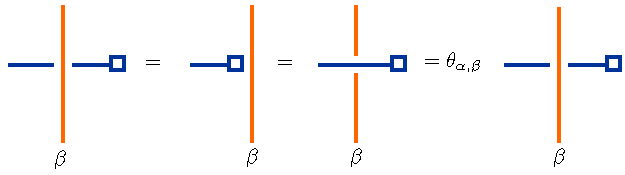
\includegraphics[scale=1]{alphabox_beta_braiding.pdf}}}},
\ee
where the orange line is a $\beta$ worldline and $\theta_{\alpha,\beta}$ is the mutual statistics of $\alpha$ and $\beta$. 
The first two equalities follow from the fact that the location of a particle being absorbed into the 
condensate is not physically significant: no operator can distinguish between states that differ only 
by the location of an $\alpha$ endpoint. 
Therefore, if $\theta_{\alpha,\beta}\neq1$, condensing $\alpha$ causes unintended collapse in $\mcc$, since it confines $\beta$.
\end{itemize}

To summarize, in order to condense $\alpha$, $\alpha$ must have a twist of 1, have bosonic self-statistics, 
and braid trivially with every other particle in the theory. 
If any of these conditions are violated, we
will have to work harder to construct $\mcc/\alpha$.



%%%%%%%%%%%%%%%%%%%%%%%%%%%%%%%
\subsection{Condensing $\psi$ in Ising} \label{condensing_psi}
%%%%%%%%%%%%%%%%%%%%%%%%%%%%%%%

In this subsection we describe our procedure for condensing $\psi$ in the Ising theory. 
While we will focus on the Ising theory in this section, our discussion will be fairly general, and can be 
applied to perform fermion condensation in more general scenarios. 

We would like to ``condense" the $\psi$ particle by constructing the quotient theory $\mcc / \psi$. 
We will denote the condensed theory by $C_2$, since the fusion rules are described by the $C_2$ Dynkin diagram; see below.
We will denote the image of $\sigma$ in the condensed theory $C_2$ as $\beta$.

First, from \eqref{psi_a_fermion}, we recall that $\psi$ is fermionic in both spin and statistics,
Additionally, we recall that $\psi$ has nontrivial braiding with $\sigma$, and as such $\psi$ is not transparent. 
Thus, $\psi$ violates all three of the conditions that particles in a condensate must satisfy! 
To condense $\psi$, we will clearly need some new tricks. 

\medskip

We will first examine how to address the non-transparency of $\psi$. 
As we saw above in \eqref{transparency_inconsistency}, 
we can't allow world lines of $\psi$ to disappear at arbitrary points in the 3-dimensional spacetime,
since this would confine $\beta$ (a.k.a.\ $\sigma$).
\be \label{box_beta_nowall_braiding}
\mathord{\vcenter{\hbox{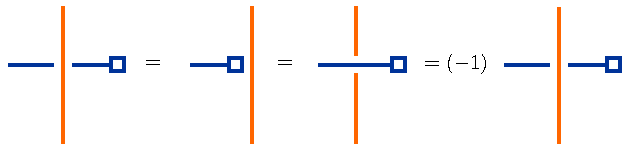
\includegraphics[scale=1]{box_beta_nowall_braiding.pdf}}}},\ee
However, if we restrict the $\psi$ worldline endpoints to lie on a 2-dimensional 
subset of the boundary of the ambient 3-dimensional spacetime,
we {\it can} obtain a consistent graphical calculus.

In this paper, we will adopt the convention that $\psi$ world lines are allowed to terminate 
on a codimension-1 ``back wall", located on a boundary of the system that is positioned ``behind'' all 
other world lines drawn in our graphical calculus. 

\begin{figure}
  \centering
    \includegraphics{Backwall_figure.pdf}
      \caption{\label{backwall} (a) The ``back wall'' picture. 
      The box represents a section of a (2+1)D Ising TQFT, with the codimension-1 back wall 
      indicated by the blue back side of the box. 
$\psi$ worldlines are absorbed into (or emitted from) the back wall at marked points labelled by $1,2,3,4$. 
Free $\psi$ endpoints which do not terminate on the back wall are not allowed. 
(b) Our way of representing the picture (a) in a (1+1)D graphical calculus. 
We have squashed the box down to a two dimensional plane, with the blue boxes representing the 
points at which the $\psi$ lines ``go straight back and hit the back wall''.}
\end{figure}

Figure \ref{backwall}(a) demonstrates this graphically, 
with the light blue back section of the box denoting the back wall, 
on which the $\psi$ worldlines can be absorbed or emitted. 
String-net graphs in our (2+1)D spacetime can be reduced to string-net graphs 
in (1+1)D spacetime by introducing a shorthand notation for $\psi$-lines terminating on the back wall. 
This notation is shown in Figure \ref{backwall}(b), 
where we use boxes to denote places where $\psi$ worldlines head straight back into the back wall and terminate.


Even though we use the same box-at-the-end-of-the-string graphical convention to denote ordinary condensation
and back wall condensation, there is an important difference.
In both cases, we can slide a box behind another strand, with the before and after pictures differing by an isotopy:
\be
\mathord{\vcenter{\hbox{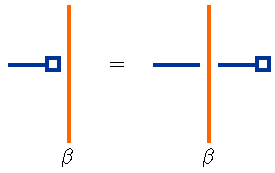
\includegraphics[scale=1]{sliding_behind.pdf}}}}.\ee
However, in the back wall case, we cannot slide a box in front of another strand
\be \mathord{\vcenter{\hbox{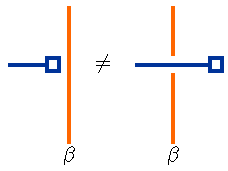
\includegraphics[scale=1]{no_sliding_above.pdf}}}}.\ee
This is because doing so would involve the other strand crossing the $\psi$ strand as it
heads into the page en route to the back wall; the before and after pictures are not isotopic.
Thus restricting $\psi$ emission/absorption to the back wall
disallows the series of diagram equalities in Figure \ref{box_beta_nowall_braiding}.

An important consequence of the existence of the back wall this is that the quotient category $C_2$ 
is not braided (although there is a way to perform the condensation so that the resulting theory is 
braided, which we mention briefly in \ref{spin_defects_condensation}).
String diagrams for braided categories (such as Ising) can be glued together in three independent 
dimensions: right/left, top/bottom, and back/front.
In more formal terms, braided categories are (special cases of) 3-categories.
Because of the back wall, it does not make sense to glue string diagrams for the $C_2$ category in the back/front
dimension.
In more formal terms, $C_2$ is a mere 2-category, or, more specifically, a (super) tensor category.
We can, however, glue an Ising string diagram to the front (but not back) of a $C_2$ diagram.
In category theoretic language, $C_2$ is a module 2-category for the Ising 3-category; equivalently, $C_2$ is a codimension 1 defect
connecting Ising to the vacuum.


\medskip

The back wall construction fixes the problems caused by $\psi$ not being transparent.
However, we have not yet addressed the spin and statistics 
inconsistencies \eqref{twist_inconsistency} and \eqref{statistics_inconsistency}.
To fix these inconsistencies, we will couple the boxes marking the $\psi$ endpoints to a 
complex line bundle associated to a spin structure. 
(When we later consider reflections, this spin structure will be promoted to a $\mbox{pin}_+$ structure.)
Readers unfamiliar with spin and pin structures are referred to Appendix \ref{spin_and_pin}. 
The spin structure will enable us to cancel out the factors of $-1$ 
arising from the endpoints of $\psi$ worldlines twisting through $2\pi$ as in \eqref{twist_inconsistency}.
This ``bosonizes'' the $\psi$ endpoints and allowing the condensation process to go through. 


\medskip

To make this precise, let $Y$ be an oriented 2-manifold, let $M = Y\times [0,1]$, and let $B = Y\times \{1\}$.
(Everything we do in this subsection will work more generally for $M$ any oriented 
3-manifold and $B$ some codimension 0 submanifold
of $\bd M$.)
In addition, choose a spin structure on $B$.
Our goal is to associate a Hilbert space to $Y$ based on string nets in $M = Y\times I$
and some extra data on the back wall $B$.

Consider the configuration space $\mcr(B)$ of all $\psi$ ribbon endpoints on $B$.
Let $\mcr(B)_k$ denote the subspace of $\mcr(B)$ corresponding to configurations with exactly $k$ endpoints.
(If $B$ is connected, then these are the connected components of $\mcr(B)$.)
We can think of the ribbon endpoint as a point $p$ of $B$ plus a tangent vector at $p$ which
points in the direction of the ``front" of the ribbon.\footnote{Ribbons 
have a distinguished front and back; if they did not, then we would have to assign
phases $\theta_a^{1/2}$ corresponding to half twists of ribbons.}
This means that $\mcr(B)_1$ is diffeomorphic to the unit tangent bundle of $B$.
We also stipulate that $\mcr(B)_0$ consists of a single point.

In the next subsection we will construct a complex line bundle $F(B)$, with flat connection, over $\mcr(B)$, 
which will provide us with the additional structure we need to perform the condensation.
The extra data alluded to above will be a vector in this vector bundle.
More specifically, for each string net $S$ in $M$, we have and endpoint configuration $e(S) \in \mcr(B)$.
Our Hilbert space will be generated by pairs $(S, v)$, where $v \in F(B)_{e(S)}$, the fiber of the bundle $F(B)$
at the configuration $e(S)$.

We impose the usual local string net relations in the interior of $M$.
(Ribbon end points are fixed for these relations.)
We also impose the following additional relation:
Let $\{S_t\}$, with $0 \le t \le 1$, be a 1-parameter family of string nets.
The $\psi$ endpoints on $B$ are allowed to move, but any other ribbon endpoints must remain fixed.
Let $v \in F(B)_{e(S_0)}$.
Using parallel translation for the connection on $F(B)$ and the path of configurations $\{e(S_t)\}$, 
we obtain $v' \in F(B)_{e(S_1)}$.
We now identify these configurations by imposing the relation
\be \label{bw_rel}
	(S_0, v) = (S_1, v') .
\ee

\medskip

Let us now see how coupling the system to $F(B)$ fixes the inconsistencies 
\eqref{twist_inconsistency} and \eqref{statistics_inconsistency}.
The crucial property of the flat connection on $F(B)$ is the the holonomies around loops
corresponding to \eqref{twist_inconsistency} and \eqref{statistics_inconsistency} is $-1$.
In other words, in \eqref{bw_rel}, we have $v = -v'$ if $\{S_t\}$ is the family of string nets
depicted in \eqref{twist_inconsistency} or \eqref{statistics_inconsistency}.

So, \eqref{twist_inconsistency} now becomes
\begin{align} \label{boxspin}
	\PsiFermion = (-1)\ \PsiFermionTwist = (-1)^2\ \PsiFermion\;. 
\end{align}
and \eqref{statistics_inconsistency} becomes
\begin{align} \label{boxbraid}
\TwoFermionNoLabels =(-1)\ \TwoFermionExchangeNoLabels = (-1)^2\ \TwoFermionNoLabels\;.
\end{align}

\medskip

Is the choice of $F(B)$ together with its flat connection uniquely determined by the above holonomy requirements?
No: in fact, there is a natural bijection between the set of spin structures on $B$ and flat connections fulfilling
the above holonomy requirements.
In other words, in order to perform this sort of fermionic condensation, we 
we need to choose a spin structure on $B$ (or on $Y$, in the main case where $M = Y\times I$ and $B \cong Y$).

\medskip

The details of the construction of the bundle-with-connection $F(B)$ are somewhat technical, 
and can be found in in Appendix \ref{flb_appendix}.
%Our discussion in the next subsection will be fairly mathematical, and physically-inclined 
%readers are invited to skip it on first reading. 
%For readers who want to skip the next subsection, we summarize some additional important facts about $F(B)$:
Some of the key properties of $F(B)$ are:
\begin{itemize}
\item In order to specify an element $v\in F(B)_{e(S)}$, it suffices to (a) assign an ordering to the $\psi$-endpoints,
and (b) choose a spin-framing at each such endpoint.
Recall that a spin structure can be thought of as a double-covering of the unit tangent bundle of $B$.
By ``spin framing" we mean a choice of lift to this double cover from the unit tangent vector determined by the ribbon orientation.
\item The most general way of specifying a spin framing is via a ``Dirac belt" connecting a base framing 
on $B$ to the tangent vector in question.
For manifolds equipped with global framings there are no ambiguities, and we can choose
a ``gauge'' in which the orientation of the belt is consistent
with the global framing, allowing us to drop the belts from the figures.
The standard Euclidean structure on a page of this paper determines a global framing (the ``blackboard framing"),
and unless stated otherwise we implicitly equip each 
$\psi$ endpoint with a spin framing determined by this choice of global framing.
In some figures we have in mind a spin structure with a different global framing,
and in these cases we will draw dashed ``branch cut" lines to indicate how the framing
differs from the standard blackboard framing. 
The branch cuts will be chosen such that 
the spin framing rotates by $2\pi$ (switches sheets on the double cover) across a branch cut. 
\item Another important property of $F(B)$ is locality: The bundles behave well with respect to gluing surfaces.
By ``behave well'', we roughly mean that for $B = B' \cup B''$, 
there is an isomorphism between $F(B)$ and $F(B')\tp F(B'')$.
\item $F(B)$ comes equipped with a way to cancel pairs of $\psi$ endpoints, which is required since the fermion 
$\psi$ we will be condensing satisfies the fusion rule $\psi \tp \psi \cong \unit$.
This requires us to supplement the parallel transport of the flat connection with additional isomorphisms of
fibers of $F(B)$ connecting points of $\mcr(B)_k$ to $\mcr(B)_{k-2}$.
\item Finally, in order to define Hermitian inner products on our Hilbert spaces, $F(B)$ comes equipped with 
an antilinear bundle map $F(B) \to F(B')$ for all orientation-reversing maps $B \to B'$.
\end{itemize}

\medskip

Our spin-structure-equipped back wall construction admits a simple physical interpretation: coupling the 
theory to the bundle $F(B)$ is equivalent to adding a phase of {\it physical} (not emergent) fermions to the theory, 
and binding single physical fermions to each $\psi$ endpoint.
The physical fermion attached to each $\psi$ endpoint compensates for the fermionic nature of the $\psi$ particle 
in the condensate: the factors of $-1$ that relate two different orderings of the $\psi$ endpoints are the Koszul 
signs associated with the physical fermions, and the factors of $-1$ that we pick up when rotating the $\psi$ 
endpoint framing by $2\pi$ come from the spin $1/2$ of the physical fermions. 
Thus, attaching physical fermions to the $\psi$ endpoints transforms them into bosonic objects, which are then 
allowed to undergo normal boson condensation. 
Therefore, although we are indeed identifying emergent fermions with the vacuum, the term ``fermion condensation'' 
is a bit misleading, as what we are actually doing is closer to {\it boson} condensation of bound states of $\psi$ 
and a physical fermion. 
However, we reiterate that the $\psi$ endpoints are not technically bosons, since they see the background spin structure: 
the emergent $\psi$ fermions do not see the spin structure, but the physical fermions attached to their endpoints do. 

\medskip

To summarize, we have seen that by introducing the back wall and equipping it with a spin structure, all three 
conditions necessary for $\psi$ endpoints to condense are satisfied.
We emphasize that we have utilized the back wall and the spin structure for two {\it independent} reasons 
(the non-transparency of $\psi$ and $\psi$'s fermionic spin and statistics, respectively). 
For example, if $\psi$ were non-transparent but bosonic, we would still need a back wall, but the back wall 
would not need a spin structure.
Conversely, if $\psi$ were transparent but fermionic, then we would not need a back wall, but we would still 
need to introduce spin
structures.


 
 
%%%%%%%%%%%%%%%%%%%%%%%%%%%%%%%%%%
\subsection{Local relations in the $C_2$ theory} \label{C2_local_relns}
%%%%%%%%%%%%%%%%%%%%%%%%%%%%%%%%%%

Now that we have worked out how to condense $\psi$, we can determine the graphical rules that govern the condensed theory. 

We have already seen that in order for the condensation procedure to go through, 
the manifold on which we define the $C_2$ theory must be equipped with a spin structure. 
The interaction of fermionic morphisms with this spin structure leads to
relations in the diagrammatic calculus that are not present in bosonic theories.  

First, we first observe that any $\psi$ strands can be absorbed into the 
condensate at the expense of phase factors, 
and so in the condensed theory the only object remaining will be the image of $\sigma$ under condensation, 
which will denote by $\beta$. 
$\beta$ lines will be drawn in orange, and $\psi$ lines will be drawn in blue (and can also be distinguished 
from $\beta$ lines through their termination points). 
In the condensed theory, the $\beta$ line may or may not have $\psi$ fermions attached to them. 
We will introduce a blue dot as a compact notation for a $\psi$ worldline that terminates on a $\beta$ line:
\be \mathord{\vcenter{\hbox{
\includegraphics[scale=1]{straight_beta_dot.pdf}}}}\quad = \quad\mathord{\vcenter{\hbox{
\includegraphics[scale=1]{straight_beta_box.pdf}}}}\ee
Note that in order for the dot notation to be unambiguous, we must specify
a spin-framing at the dot.
We will usually do this implicitly as follows.
The dots are only allowed to occur on vertical strands,
and the spin framing at the dot is obtained from the base framing of the manifold
by rigidly translating with respect to the ``blackboard framing" of the page.
For diagrams which do not inherit their spin structure from the blackboard,
we will have to use other means to specify the spin-framing.
\kw{the above discussion needs improvement}
%Note that in order for the dot notation to be unambiguous, the dots can only occur on
%vertical strands, and the diagram should have an implicit framing. 
%We usually take this to be the ``backboard framing'' 
%inherited from the inclusion of the diagram into $\mathbb R^2$ (the blackboard).
%We will depart from this convention when the surfaces on which our diagrams live
%possess non-bounding spin structures, and in these cases we will indicate departures
%from the blackboard framing convention by drawing branch cuts in figures. 

Because $\beta$ lines in the condensed theory can have fermionic dots on them, 
there are several new diagrammatic rules involving them that need to be included in our graphical calculus. 
One of the most important local relations is 
the addition and removal of an even number of fermions on $\beta$ lines. 
The process of removing two fermions can be done at the cost of a phase factor: 
\begin{align} \label{removing_fermions}
\mathord{\vcenter{\hbox{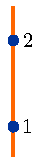
\includegraphics[scale=1]{beta_dotdot.pdf}}}} \quad =  \quad \mathord{\vcenter{\hbox{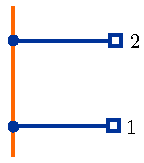
\includegraphics[scale=1]{beta_boxbox.pdf}}}} \quad = \quad 
\mathord{\vcenter{\hbox{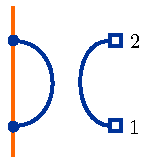
\includegraphics[scale=1]{beta_curvy_boxbox.pdf}}}} \quad =\quad  
\lambda\; \mathord{\vcenter{\hbox{
\includegraphics[scale=1]{straight_beta.pdf}}}}\;,
\end{align}
where the labels $1$ and $2$ denote the 
ordering of the fermions in question.
We have performed an $F$-move on the $\psi$ worldlines to get the second equality, 
used \eqref{Ising_bubble_relns} 
to remove the $\psi$ line attached to the $\sigma$ line in the third diagram, 
and have used  
\be \label{eval_psi_semicirc}
   \PsiEnd  = \lambda \times \text{(vaccuum)},
\ee
in the last step to remove the semicircular $\psi$ line, where $\lambda\in \cc$ is some complex number. 
\kw{should probably move this (above) to previous subsection.  KW will take care of it.}
We show in Appendix \ref{flb_appendix} that we must have $\lambda=\pm i$, and since $A^4=\pm i$ in the Ising theory, 
we may choose either $\lambda = A^4$ or $\lambda = -A^{4}$ (the choice of $A$ does not constrain the choice of $\lambda$).  
The choice of $\lambda = \pm A^4$ affects the $F$-symbols in the condensed theory, 
but does not affect observable quantities like the twists or mutual statistics of the 
quasiparticles in the theory\footnote{This is because the choice of $\lambda=\pm A^4$ doesn't 
change the ``multiplication table'' of the tube category, which we will discuss below. 
Essentially, changing $\lambda$ just performs a scaling on the $\psi$ endpoints in the figures.}.
Therefore without loss of generality we may choose a gauge in which $\lambda=A^4$, and so 
\begin{align}  \label{removing_fermions}
\mathord{\vcenter{\hbox{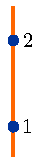
\includegraphics[scale=1]{beta_dotdot.pdf}}}} \quad = A^4\; \mathord{\vcenter{\hbox{
\includegraphics[scale=1]{straight_beta.pdf}}}}\;,
\end{align}


Since $\psi$ is statistically fermionic, exchanging two fermions on a $\beta$ line results in a minus sign:
\begin{align}
\mathord{\vcenter{\hbox{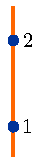
\includegraphics[scale=1]{beta_dotdot.pdf}}}} \quad = \quad (-1)\times
\mathord{\vcenter{\hbox{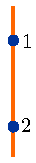
\includegraphics[scale=1]{beta_dotdot_switched.pdf}}}}\;.
\end{align}
%%KW: the following discussion seems unnecessary (and also a little confusing) to me
%In order to account for all statistical signs like this correctly, 
%when we annihilate a pair of dots using \eqref{removing_fermions}, 
%we must be careful to only annihilate pairs that have the same ordering as they did when they were created, 
%so that their orders are adjacent to one another.
%For example, if we create a pair of dots using \eqref{removing_fermions} in a 
%configuration where the upper fermion has order $m$ and the lower fermion has order $n$, 
%we must be careful to only annihilate them when they are in this configuration. 
%Failing to follow this rule will result in diagrams possessing erroneous minus signs. 


The braiding in the parent Ising theory means that we pick up non-trivial phase 
factors when sliding fermion dots over and around $\beta$ caps and cups. 
For example, we can compute
\begin{align} \label{capslide}
\capleftdot =
\mathord{\vcenter{\hbox{
\includegraphics[scale=1]{cap_left_box.pdf}}}} =
\mathord{\vcenter{\hbox{
\includegraphics[scale=1]{cap_left_through_box.pdf}}}} =
\mathord{\vcenter{\hbox{
\includegraphics[scale=1]{cap_right_twist_box.pdf}}}}
= A^4 \caprightdot,
\end{align}
where in the last step we have used \eqref{sig_psi_Rsymbol}. 
Since in the Ising theory $A^4=\pm i$, we can invert \eqref{capslide} to find 
\begin{align} \label{cap_slide_back}
\caprightdot\; &= - A^4 \; \capleftdot.
\end{align}
By a similar argument we find
\be  \cuprightdot\; =  A^4 \; \cupleftdot\;. \ee
Because of the nontrivial rules for sliding dots through cups and caps, dots which live 
on the apex of a cup or the bottom of a cap (where the $\beta$ line is horizontal) are ambiguous, 
and we will not allow them to be drawn in our fusion diagrams.

We stress that these phases are derived completely from the {\it braiding data} of the Ising theory. 
%They also must be such that taking a fermion dot around a circular $\beta$ loop gives a factor of $-1$, 
%which enforces the constraint that $A^8 = -1$. 

Note that the above relations imply that even-parity $\beta$ loops are non-zero, while odd-parity $\beta$ loops vanish:
\be \mathord{\vcenter{\hbox{
\includegraphics[scale=1]{beta_circle.pdf}}}}=0 .\ee
This is as expected -- dragging the fermionic dot around the circle rotates it through $2\pi$.
%which can be easily seen by dragging the dot once around the circle. 
%The fact that $A^8=-1$ must also be true because dragging the fermion once around the circle 
%amounts to a $2\pi$ rotation of the fermion framing, which must be equivalent to multiplication by $-1$. 
%The constraint $A^8=-1$ is satisfied in all the Ising theories. 
%However, in more general examples this constraint on the braiding data is a strong one, 
%and significantly limits the types of theories that can have objects with $\cl_1$ 
%endomorphism algebras capable of ``absorbing'' fermions.


The final local relations that will be important in what follows are the $F$-moves, 
which provide linear relations between different isotopy classes of diagrams.
The $F$-symbols in the condensed $C_2$ theory can be worked out using our rules 
for manipulating condensed $\psi$ worldlines and our knowledge of the $F$-symbols 
in the parent Ising theory.
We begin with a diagram in the Ising theory, apply an $F$-move, 
and then remove all $\psi$ lines through condensation to evaluate the $F$-move in the $C_2$ theory. 
For example, in the parent Ising theory we have
\begin{align}
\doublebeta = \frac{1}{d} \left(\doublecups + \doublecuppsi\right).
\end{align}
When we condense $\psi$, the second diagram on the left hand side becomes 
\be \label{fmove_isingtoC2}
\doublecuppsi = A^{-4}\; \mathord{\vcenter{\hbox{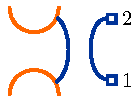
\includegraphics[scale=1]{double_cup_psi_line_wsemicircle.pdf}}}}\; \mapsto A^{-4}\;
\doublecupdots\;. \ee
Note that in the first step of \eqref{fmove_isingtoC2} we have displaced the 
vertical $\psi$ line to the right, so that it never intersects the $\beta$ line at 
the apex of a cap or the bottom of a cup.
We do this to avoid ambiguities in the fermion framing, 
which as discussed earlier always points ``to the left'', 
meaning that dots living on horizontal $\beta$ lines are not well-defined. 
While we choose to displace the $\psi$ line to the right in \eqref{fmove_isingtoC2}, 
this is merely a gauge choice: we could have equally well chosen it to be displaced to the left. 
Recapitulating, we see that in the $C_2$ theory we have the $F$-move
\be \doublebeta\; = \frac{1}{d} \left( \doublecups \; + \;A^{-4} \doublecupdots\right).
\label{Fmove}\ee
By similar reasoning we can derive the other nontrivial $F$-move in the $C_2$ theory, which is
\begin{align} \label{cupcap_fmove}
\doublecups\; &= \frac{1}{d} \left(\doublebeta \; + \; \doublebetadots \right).
\end{align}

The fact that $\beta$ lines can host dots means that $\beta$ has an endomorphism which 
is not a multiple of the identity, 
which is a hallmark of physics that cannot be found in bosonic topological phases. 
Indeed, any section of a given $\beta$ worldline may look like
\begin{align} \label{betaendos}
\mathord{\vcenter{\hbox{
\includegraphics[scale=1]{straight_beta.pdf}}}} \qquad {\rm or} \qquad \mathord{\vcenter{\hbox{
\includegraphics[scale=1]{straight_beta_dot.pdf}}}}.
\end{align}
The two diagrams in \eqref{betaendos} are the generators of the endorphism algebra of $\beta$.
Since we have one even generator and one odd generator we see that $\text{End}(\beta) \cong \mathbb{C}\ell_1$, 
where $\cl_1$ is the first complex Clifford algebra (generated by $1$ and a single odd-parity generator). 
More generally, the vector space assigned to a disk with $2n$ $\beta$ strings ending on its boundary is 
has dimension $2^n$, and the endomorphism algebra of $\beta^{\tp n}$ (i.e.\ $n$ copies of $\beta$ on a line) is
isomorphic to $\cl_n$.

In more general contexts, we will refer to simple objects whose endomorphism algebras are isomorphic 
to $\cl_1$ as ``q-type objects'', and those whose endomorphism algebras are isomorphic to $\cc$ 
as ``m-type objects''. 
From the above information, we can infer the fusion rule
\be \beta\tp\beta \cong \cc^{1|1} \cdot \unit, \ee
where $\cc^{1|1}$ is the complex vector space with a single even generator and a single odd generator, 
corresponding to the even and odd channels of the fusion product $\beta\tp\beta$. 


In bosonic theories, having $\End(\beta)\cong\cl_1$ would imply that $\beta$ is not a simple object, 
since by Shur's lemma the endomorphism algebra of any simple object must be a division algebra, and
since $\cc$ is the only ungraded division algebra.
Nevertheless, $\beta$ {\it is} a simple object\footnote{Indeed, if we tried to decompose $\beta$ 
into two idempotents, they would each be linear combinations of the two pictures in \eqref{betaendos}, 
which have different fermion parity.
But idempotents must have even parity.}
%Since diagrams with different fermion parities are in different superselection sectors, 
%we are not allowed to add them together to form linear combinations, which is a contradiction.}.
This is possible because in fermionic theories, the Hilbert spaces we use are supervector spaces, 
compared to the regular vector spaces of bosonic theories. 
Unlike in the bosonic case, there are {\it two} super division algebras, $\cc$ and $\cl_1$.
This means that simple objects in the fermionic setting can have endomorphism algebras of either $\cc$ or $\cl_1$.  
Later on, we will see that the existence of simple objects with $\cl_1$ endomorphism 
algebras is responsible for a large part of the novel physics that occurs as a result of fermion condensation. 

Finally, we mention a higher-level way of understanding the content of the $C_2$ theory from the
parent Ising theory. We begin by noting that the principle graph for the Ising theory 
is given by the $A_3$ Dynkin diagram (see the top left of Table \ref{C2_data_table}). 
Condensing $\psi$ means establishing an isomorphism between $\psi$ and $\unit$, 
so that in the condensed theory $\unit$ and $\psi$ correspond to the same node of the 
principal graph. This identification can be done by ``folding'' the $A_3$ principal graph 
about the central node so that the $\unit$ and $\psi$ nodes are identified. 
Note that $\sigma$ is preserved under the folding, which translates into the fact that the 
image of $\sigma$ in the condensed theory (namely $\beta$) has a nontrivial endomorphism 
algebra. 
The resulting folded principal graph is shown in the top right of Table \ref{C2_data_table}: the double 
line indicates the two fusion channels in $\beta\tp\beta \cong\cc^{1|1}\cdot \unit$, the 
double circle indicates that $\beta$ has a two-dimensional endomorphism algebra, and 
the arrows have been chosen to point away from the object with larger endomorphism 
algebra. The resulting principal graph is precisely the $C_2$ Dynkin diagram, 
which is why we call the condensed theory the $C_2$ theory. 
This idea can be applied to perform fermion condensation in many other theories (most straightforwardly 
the other theories in the $A_n$ series which contain a fermion). 
We will explore several examples along these lines in later sections. 



\begin{table}
	\fbox{\begin{minipage}{148mm}
	\vspace{3mm}\begin{center}{\begin{minipage}{128mm}
		\setlength{\parskip}{0ex}
		\begin{align*}
		\xymatrix @!0 @M=4mm @R=6mm @C=60mm {
		 \AThreeDynkin \ar@<7pt>[r]^{\text{condense $\psi$}}&   \CTwoDynkin
		 }
		\end{align*}
		
		\textbf{Basic data:}\\[-4ex]
\begin{flalign*} & \begin{array}{c @{\quad \quad  } c @{\quad \quad } c @{\quad \quad } c}
			\text{simple objects}	&	\text{fusion rules} &   \text{dimensions} & \text{Koszul signs}
		\\[.5ex]
			\text{$\unit$ and $\beta$}
			&	 \beta \tp \beta \cong \mathbb{C}^{1|1}\cdot \mathds{1}  & \dbeta_\beta  = d &  \SigmaDotDot = - \SigmaDotDotExchange
		\end{array} & \end{flalign*}
\vspace{3mm}
		\textbf{Linear relations:}\\[-4ex]
		\begin{flalign*} & \begin{array}{r @{\quad \quad} l @{\quad \quad} l @{\quad \quad} l}
			\text{F-symbols}
			&	d\;  \TwoLine =  \CupCap  +A^{12}\CupCapDots  & d\; \CupCap =\TwoLine + \TwoLineDots
				&	\eqref{Fmove}
		\\[4ex]
			\begin{tabular}{c}Fermion\\ pairing\end{tabular}
			&	\;\;  \SigmaDotDot = A^4\; \FubeXss \quad  \eqref{removing_fermions} & \; \begin{tabular}{l}$\CapDotLeft =  A^4 \CapDotRight$ \\ \\$ \CupDotRight = A^{4} \CupDotLeft $ \end{tabular}
				&	\eqref{cap_slide_back}
			\end{array} & \end{flalign*}
			 $A^2 = - e^{\pm i \pi /4}$ \quad \quad $d  = -A^2 - A^{-2}$ \quad  \eqref{QuantumDimensions}
	\end{minipage}}\end{center}\vspace{1mm}
	\end{minipage}}
	\caption{Summary of $C_2$ data}  \label{C2_data_table}
\end{table}

